\documentclass[a4paper,twosided,12pt,DIV12]{scrartcl}
%
% all the local settings defined in /localsettings.sty
\usepackage{localsettings}
\usepackage{customsymbols}
%
% lazyeqn - math symbols
% Uncomment if you have chosen to clone it to your project
\usepackage{./lazyeqn/lazyeqn}
\addtokomafont{disposition}{\rmfamily}
%
\usepackage{scalefnt}

\newcommand\smallerr[2][0.85]{{\scalefont{#1}#2}}

\newcommand\ilabel[1]{I\smallerr{#1}}
% \usepackage{accents}

% \newcommand\ub[1]{%
%   \underaccent{\bar}{#1}}

% \makeatletter
% \def\ub#1{\underline{\sbox\tw@{$#1$}\dp\tw@\z@\box\tw@}}
% \makeatother

\DeclareMathOperator{\ivt}{ivt}
\DeclareMathOperator{\idxop}{idx}
\DeclareMathOperator{\per}{per}
\DeclareMathOperator{\rank}{rank}
\DeclareMathOperator{\ifop}{if}
\DeclareMathOperator{\invop}{inv}

% \makeatletter
% \newcommand{\idxop}{\mathop{\operator@font idx}}
% \newcommand{\per}{\mathop{\operator@font per}}
% % \newcommand{\ivt}{\mathop{\operator@font ivt}}
% \newcommand{\rank}{\mathop{\operator@font rank}}
% \newcommand{\ifop}{\mathop{\operator@font if}}
% \newcommand{\invop}{\mathop{\operator@font inv}}
% \makeatother

\newcommand{\veps}{\vareps}

% \def\ub#1{\underline{\smash{#1}}}
\def\ub#1{\underline{#1}}

% \newcommand{\idx}[1]{#1_1 #1_2 \dotsm #1_N}
% \newcommand{\idxu}[1]{\ub{#1}_1 \ub{#1}_2 \dotsm \ub{#1}_N}
% \newcommand{\idxn}[2]{#1_1 #1_2 \dotsm #1_{#2}}
% \newcommand{\idxnu}[2]{\ub{\idxn{#1}{#2}}}

\newcommand{\idx}[1]{#1_1 \dotsm #1_N}
\newcommand{\idxu}[1]{\ub{#1}_1 \dotsm \ub{#1}_N}
\newcommand{\idxn}[2]{#1_1 \dotsm #1_{#2}}
\newcommand{\idxnu}[2]{\ub{\idxn{#1}{#2}}}

%
\frenchspacing
%
% \title{Array Calculus}
\title{Composites Modeling WS2014--2015 Assignment}
\author{Huseyin Onur Solmaz -- Matr.2868402}
\date{}
%



\begin{document}
\maketitle

\section{Estimation of Material Constants (Task 1)}

The following tables give typical mechanical data for T300 carbon-fiber and
Hexcel 8551-7 epoxy resin.

\begin{table}[H]
  \centering
  \begin{minipage}{0.45\textwidth}
    \footnotesize
  \begin{tabular}{p{0.7\textwidth}p{0.2\textwidth}}
    \toprule
    Fiber type & T300\\
    Longitudinal modulus $E_{11}$ (GPa) & 231\\
    Transverse modulus $E_{12}$ (GPa) & 15\\
    Transverse modulus $E_{13}$ (GPa) & 15\\
    In-plane shear modulus $G_{f12}$ (GPa) & 15\\
    Major Poisson's ratio $\nu_{f12}$ & 0.2\\
    Major Poisson's ratio $\nu_{f13}$ & 0.2\\
    Transverse shear modulus $G_{f23}$ (GPa) & 7\\
    Longitudinal tensile strength $X_{f1T}$ (MPa) & 2500\\
    Longitudinal compressive strength $X_{f1C}$ (MPa) & 2000\\
    Longitudinal tensile failure strain $\veps_{f1T}$ (\%) & 1.086\\
    Longitudinal compressive failure strain $\veps_{f1C}$ (\%) & 0.869\\
    \bottomrule
  \end{tabular}
  \end{minipage}
  \begin{minipage}{0.45\textwidth}
    \footnotesize
  \begin{tabular}{p{0.7\textwidth}p{0.2\textwidth}}
    \toprule
    Matrix type & 8551-7 epoxy\\
    Elastic modulus $E_{m}$ (GPa) & 4.08\\
    Elastic shear modulus $G_{m}$ (GPa) & 1.478\\
    Elastic Poisson's ratio $\nu_{m}$ (GPa) & 0.38\\
    Tensile strength $Y_{mT}$ (MPa) & 99\\
    Compressive strength $Y_{mC}$ (MPa) & 130\\
    Shear strength $S_{m}$ (MPa) & 57\\
    Tensile failure strain $\veps_{mT}$ (\%) & 4.4\\
    Compressive failure strain $\veps_{mC}$ (\%) & 9\\
    Shear failure strain $\gamma_{m}$ (\%) & 5.1\\
    \bottomrule
  \end{tabular}
  \end{minipage}
\end{table}
\subsection{Estimation (Part a)}

\textit{Use necessary micro-mechanics formulae to estimate elastic modulus (E11, E22,
G12), Poisson's ratios (V12 and V21) and failure properties for maximum stresses
(F11T, F11C, F22T, F22C and F12=F6) assuming the composite is unidirectional
with \textbf{a fiber volume ratio of 50\%}}

\subsection{Discussion (Part b)}

\textit{Briefly discuss the limitations of micro-mechanics to predict mechanical
properties, especially failure properties.}


\section{}
\textit{This uni-directional composite is used for a simple square flat plate as shown
below having a length of 400mm and with 300mm. Eight plies having a symmetric
lay-up [0/90/+45/-45]s are used. Assume the ply thickness is 0.25mm and the
0\degree fiber direction is in the plate length (x) direction.
\\The composite plate has a line load as shown and is simply supported at both
ends in the width direction.}

\begin{center}
  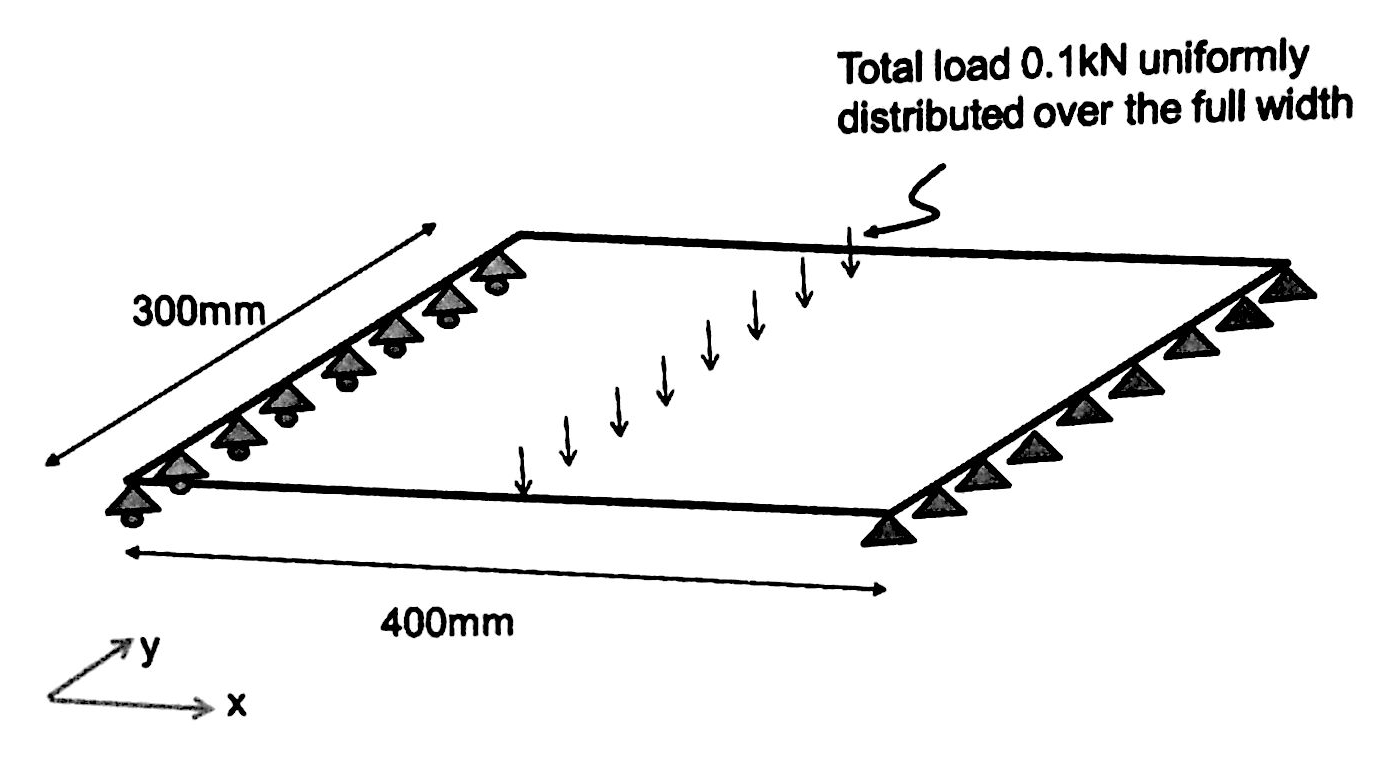
\includegraphics[width=0.7\textwidth]{fig1.png}
\end{center}

\subsection{}

\textit{Use laminate analysis to compute the relevant laminate stiffnesses and classical
beam bending formulae to estimate maximum deflection at the center of the
plate.}

\subsection{}

\textit{Use laminate analysis and the failure data from question 1, to estimate the
first and last ply failure loads.}

\section{}

\textit{Create a Finite Element model of the above problem having identical
boundary conditions, loadings and material properties.
\\Perform an implicit Finite Element analysis and compute the central
deflection. Copmare results with the previous classical solution using laminate
analysis.}

\section{}

\textit{Modify the above finite element model to include two geometric stiffeners (so
called Beads or Sikkens). Choose a suitable spacing for the sickens with each
one having approximate dimensions of 250mm length and 30mm with (15mm height).
Note a useful option exists in Visual Mesh for this operation (2D > Bead on 2D mesh).
The plate with Sikkens has identical loading (line load across the center) and
boundary conditions identical to question 2.}

\begin{center}
  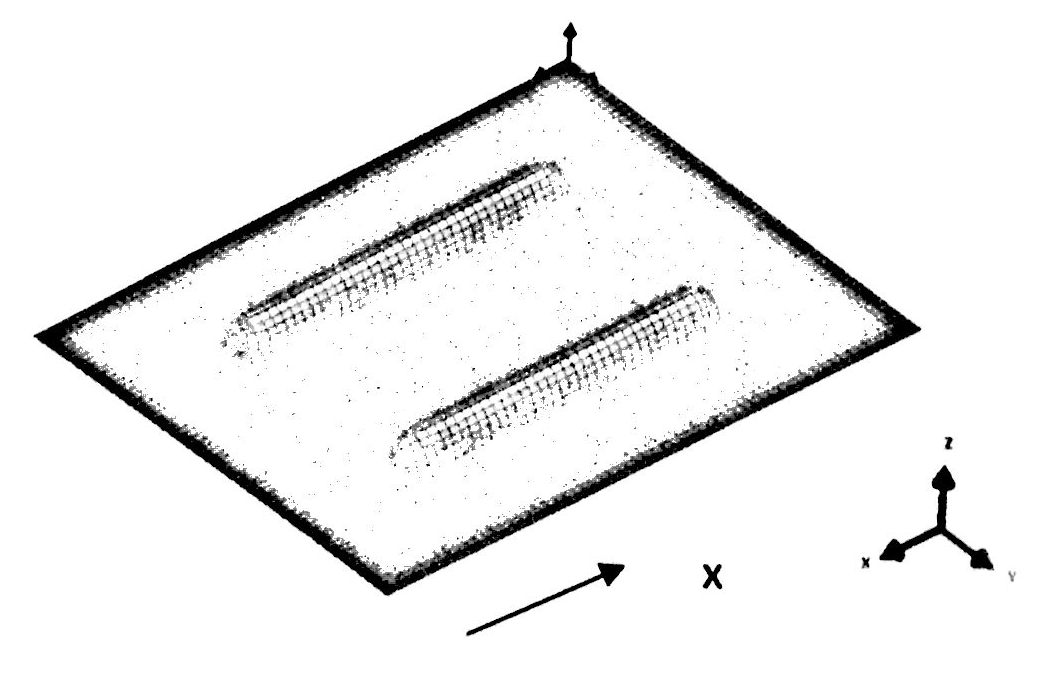
\includegraphics[width=0.7\textwidth]{fig2.png}
\end{center}

\textit{Use the ILAY=1 option to define the laminate, which has the same materials,
lay-up orientations and ply thicknesses as used in questions 2 and 3. Define
Auxiliary 26 to get the failure load indicator for all plies (done in the
material cards). For the output contours to work properly, you will need to use
the ILAY=1 option and also visualize results from the .erfh5 file (for erf5 file
output set ERFKEY=3 in the OCTRL control card).}

\textit{Perform an implicit failure analysis of the plate with Sikkens and compute
\begin{enumerate}
\item The maximum deflection.
\item The failure load using a maximum stress criterion and the composite
  failure data determined from question 1.
\item From the contour results for ``Ply Failure Criteria'' estimate the
  necessary applied load to just cause first ply failure of the structure.
\end{enumerate}}

\section{}
%
\textit{Perform a PAM-RTM infusion simulation of the Plate with Sikkens.
\\Beware that PAM-RTM uses only triangular shell elements and the units should
be in meters, if you want to be consistent with default data provided in
PAM-RTM. Both element type (option MESH > TRANSFORM > SPLIT QUADS...) and units
(option MESH > TRANSFORM > SCALE...) can be converted in PAM-RTM, or in Visual
Mesh with similar options.
\\Assume the resin inlet is as shown below. Use pressure injection with 1 bar
difference between inlet and outlet. Assume the infusion is isothermal at room
temperature and the fabric has isotropic permeability throughout.}
%
\begin{table}[H]
  \centering
  \begin{tabular}{ll}
    Thickness of composite & 2 mm\\
    Resin viscosity at 23\degree C & 0.3 Pa sec \\
    Assume PAM-RTM standard fabric with porosity & 0.5 \\
    Fabric permeability & 1E-10 m\textsuperscript{2}\\
  \end{tabular}
  \caption{Infusion and other data}
\end{table}
%
\begin{center}
  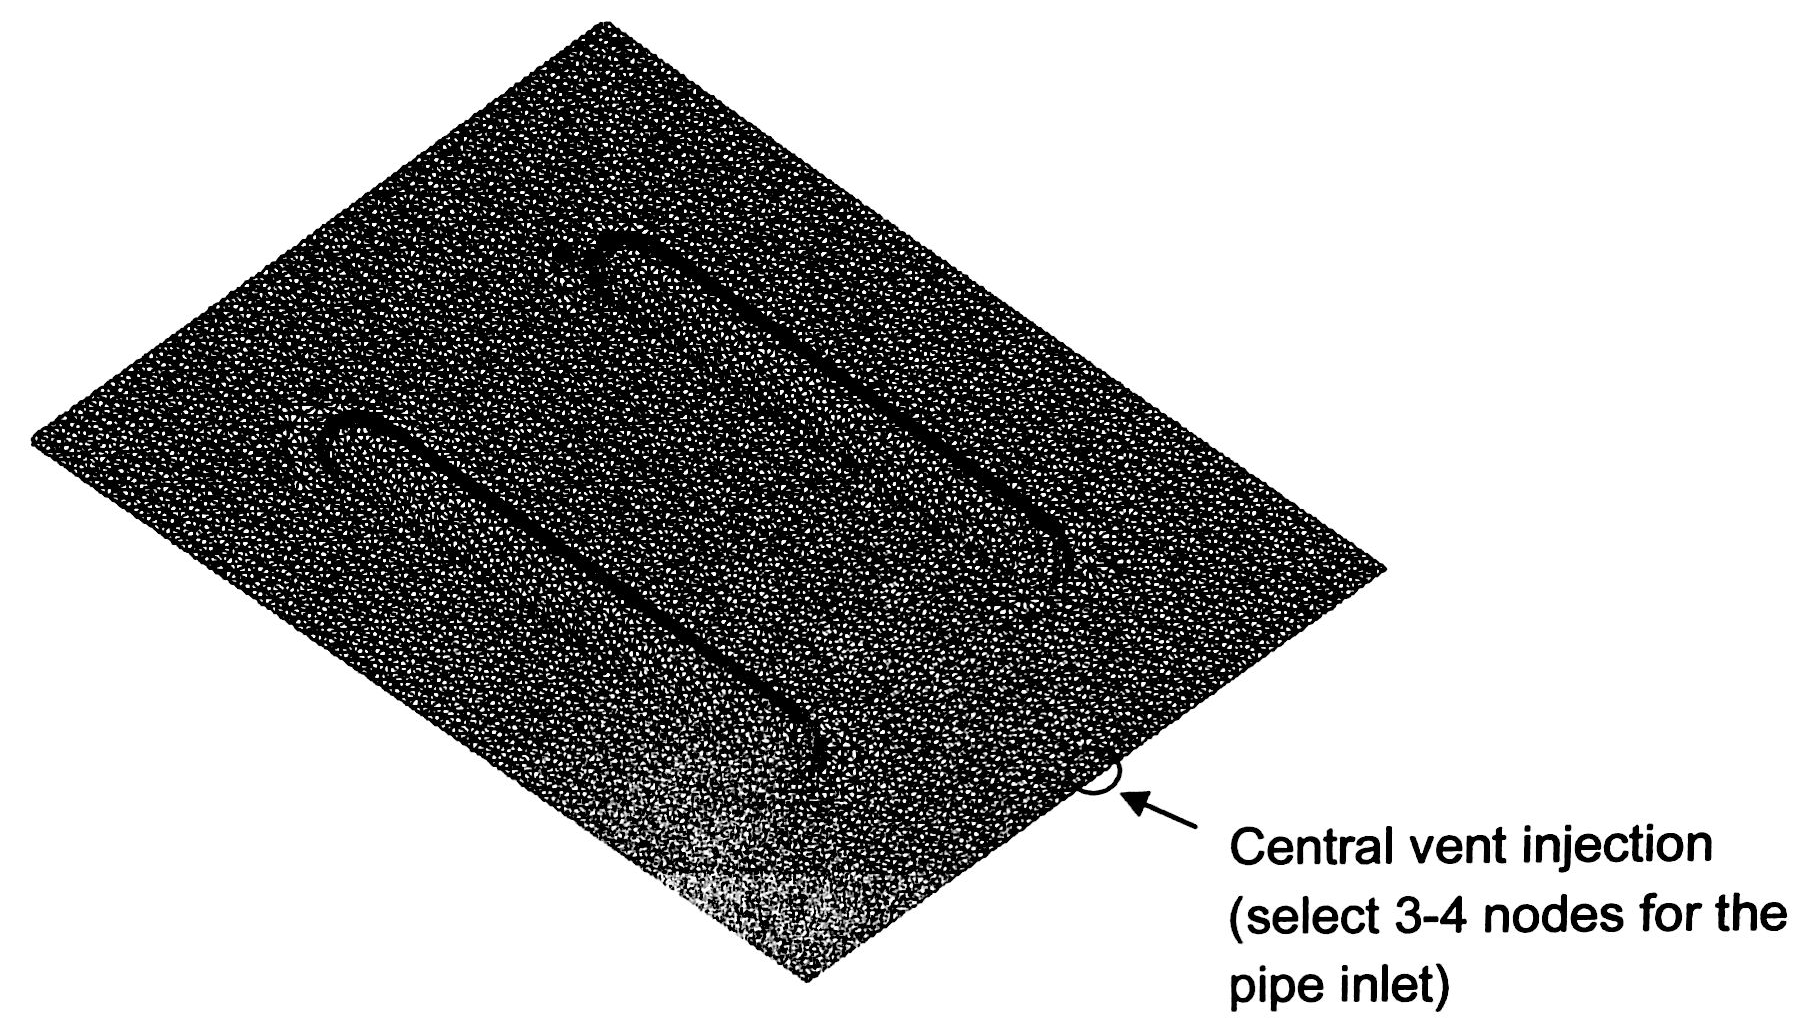
\includegraphics[width=0.7\textwidth]{fig3.png}
\end{center}
%
\textit{Perform an RTM type analysis and estimate:
%
\begin{enumerate}
\item The time for infusion and suitable positions for the outlet vents.
\item If the resin is known to gel after 30 minutes, is the infusion likely to
  be successful?
\item Propose and try an alternative infusion strategy with a view to speeding
  up the infusion time and having a good infusion. Where should the outlet vents
  be placed for your chosen setup?
\end{enumerate}}


\end{document}
%
